\documentclass[12pt,a4paper]{article}
\usepackage[utf8]{inputenc}
\usepackage[english,russian]{babel}
\usepackage{amssymb,amsfonts,amsmath,cite,enumerate,float,indentfirst}
\usepackage{graphicx}
\graphicspath{{images/}}
\usepackage{geometry}
\usepackage{systeme}
\usepackage{hyperref}
\usepackage{url}
\usepackage{mathtools}
\usepackage{slashbox}
\usepackage{multirow}
\usepackage{csquotes}
\usepackage{subfigure}
\hypersetup{
	colorlinks,
	citecolor=black,
	filecolor=black,
	linkcolor=black,
	urlcolor=black
}
\geometry{left=2cm}
\geometry{right=1.5cm}
\geometry{top=2cm}
\geometry{bottom=2cm}

\begin{document}
	\begin{titlepage}
		\begin{center}		
			\vfill	
			Санкт-Петербургский политехнический университет \\
			Петра Великого\\
			\vskip 1cm
			Институт прикладной математики и механики \\
			Кафедра «Прикладная математика»
			\vfill
			\textbf{Отчёт\\
			по курсовому проекту\\
			по дисциплине\\
			«Методы оптимизации»\\}
			\vfill
		\end{center}
		\vfill
		\hfill
		\begin{minipage}{0.4\textwidth}
			Выполнил студент:\\
			Петрунин Григорий Дмитриевич\\
			группа: 3630102/70201\\
		\end{minipage}
		\vfill
		\hfill 
		\begin{minipage}{0.4\textwidth}
			Проверил(a):\\
			к.ф.-м.н.\\
			Родионова Елена Александровна\
		\end{minipage}
		\vfill
		\begin{center}
			Санкт-Петербург\\2020 г.
		\end{center}
	\end{titlepage}

	\tableofcontents
	\listoffigures
	
	\newpage
	
	\section{Постановка задачи}
		Задача ставится в терминах двумерной идеальной модели следующим образом:\\
		Имеется канал заданной ширины с прямоугольным поворотом. Имеется твердое тело - плот, конфигурация которого представляет следующую фигуру: \textit{квадрат, одна из сторон которого является диаметром полукруга}. Необходимо вычислить параметры плота, отвечающие  максимальной его площади, с которой он сможет пройти этот поворот.\\
	
	\section{Предварительный анализ}
		Для начала приведем необходимые графические представления исходных данных задачи.
		
		\subsection{Конфигурация плота}
			Исходное описание позволяет нам построить следующую модель:
			\begin{figure}[H]\label{fig:sofa}
				\centering
				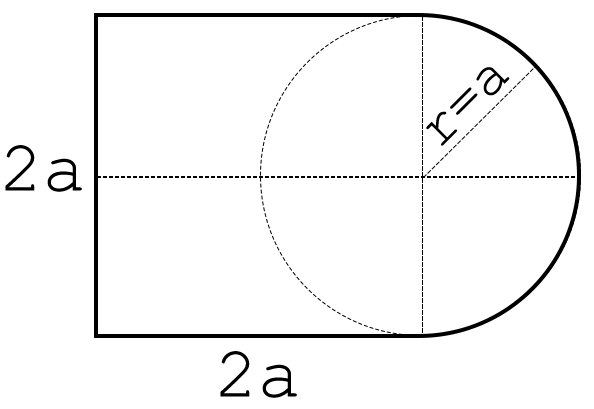
\includegraphics[width=6cm]{res/sofa.png}
				\caption{Схема плота}
			\end{figure}
			Ясно, что единственным параметром плота, который мы будем искать в этой задаче, будет радиус полукруга $a$, он же половина линейного размера квадрата. В таком случае искомым значением площади будет
			\begin{equation}\label{eq:area}
				S = 4a^2 + \frac{\pi a^2}{2}
			\end{equation}
			
		\subsection{Схематический рисунок задачи}
			Приведем иллюстрацию поставленной задачи для наглядности:
			\begin{figure}[H]\label{fig:scheme}
				\centering
				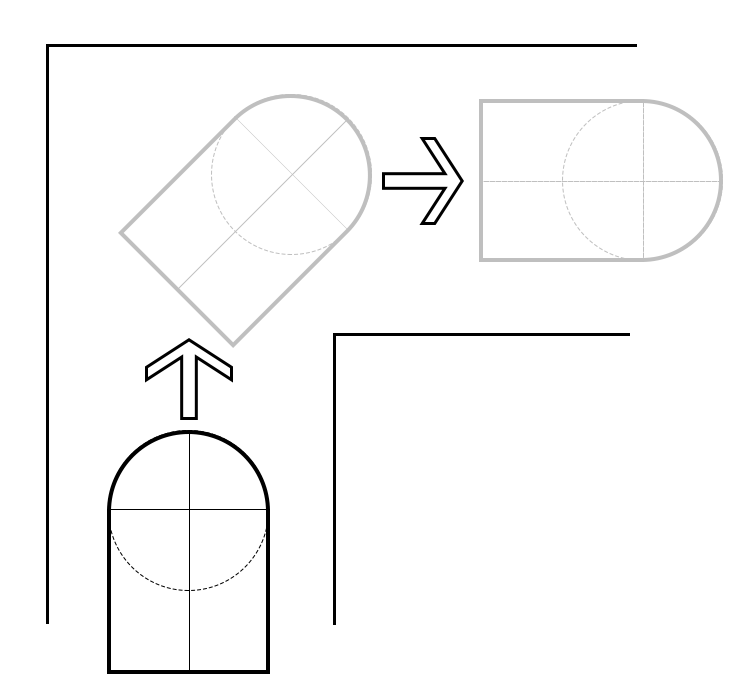
\includegraphics[width=6cm]{res/scheme.png}
				\caption{Схема задачи}
			\end{figure}
		
		\subsection{Вспомогательные утверждения}
			Перед тем, как браться за формализацию задачи, установим пару простых идей, которые нам помогут:
			\begin{itemize}
				\item Очевидно, что при попытке продвижения плота через поворот его начальное положение следует выбирать так, чтобы его ось симметрии была параллельна стенкам канала (как на \hyperref[fig:scheme]{\textit{Рис.2}}). Движение плота на прямых участках в положении поперек заблаговременно позволит нам найти лишь приближенное решение $a = \frac{w}{3}$, как продемонстрировано на следующей схеме:
				\begin{figure}[H]\label{fig:example}
					\centering
					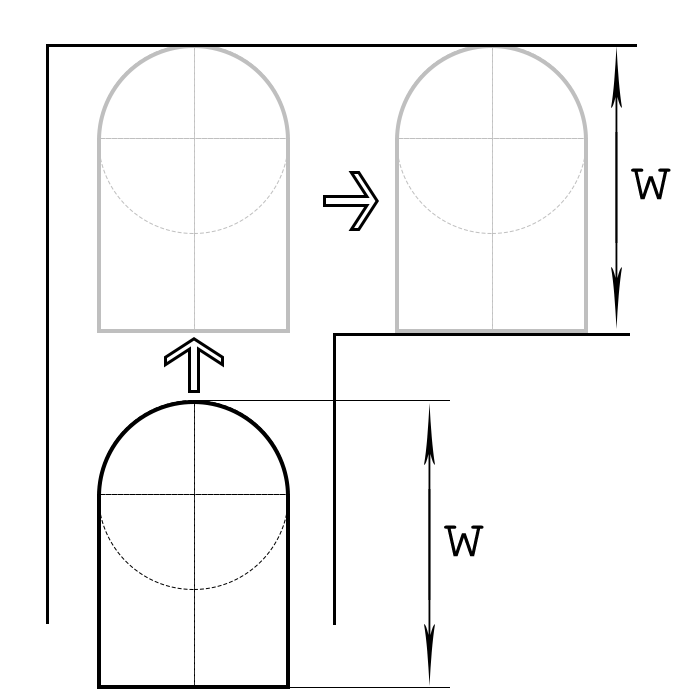
\includegraphics[width=6cm]{res/example.png}
					\caption{Пример приближенного решения}
				\end{figure}
				
				\item Из предыдущего пункта следует, что у нас остается 2 варианта, как задавать начальное положение плота: полукругом вперед, как на \hyperref[fig:scheme]{\textit{Рис.2}}, либо полукругом назад. Очевидно, что оба варианта эквивалентны в силу симметрии, поэтому для нашей задачи будем рассматривать движение полукругом вперед.
				
				\item \textit{Замечание:} опять же в силу симметрии очевидно, что решение данной задачи позволит нам продвигать плот найденной конфигурации в каналах с поворотами в другую сторону в отличие от, например, фигуры найденной Джоном Хаммерсли в 1968г. для т.н. \hyperref[1]{\textit{Задачи о диване} [1]}.
			\end{itemize}
		
	\section{Формализация задачи}
		Теперь когда мы определились, каким именно образом мы будем продвигать плот через поворот в канале, можно попытаться формализовать нашу задачу.\\
		\vskip 0.1 cm
		Во-первых, очевидно, что задача относится к оптимизационным и имеет функцию цели
		\begin{equation}
			a \longrightarrow max
		\end{equation}
		Однако, данная работа носит скорее исследовательский характер, поэтому приближенное решение мы будем находить экспериментально. Тем не менее, алгоритмами оптимизации мы все же воспользуемся.
		
		\subsection{Ограничения}\label{subsec:limitations}
			Единственной искомой переменной задачи является параметр ее размера $a$, на который необходимо наложить разумные ограничения, в пределах которых мы будем искать нужное значение. За такие ограничения можно взять, например, промежуток $(\frac{w}{3}, \frac{w}{2})$, где $w$-ширина канала. Левая его граница, как мы уже выяснили, соответствует начальному приближению, см. \hyperref[fig:example]{\textit{Рис.3}}. Правая граница соответствует максимально возможному начальному положению плота на прямом участке канала.
		
		\subsection{Анализ модели}
			В этой работе мы будем максимально упрощать математическую модель перемещения двумерного тела. Для этого нам необходимо понять, какие именно ограничения встречает плот при попытке войти в поворот.\\
			
			При достаточных размерах плота экспериментальным путем (на самом деле благодаря наглядности задачи этот факт можно установить воспользовавшись лишь пространственным воображением) устанавливается, что для преодоления поворота плот встречает 3 препятствия. Приведем схему:
			\begin{figure}[H]\label{fig:edges}
				\centering
				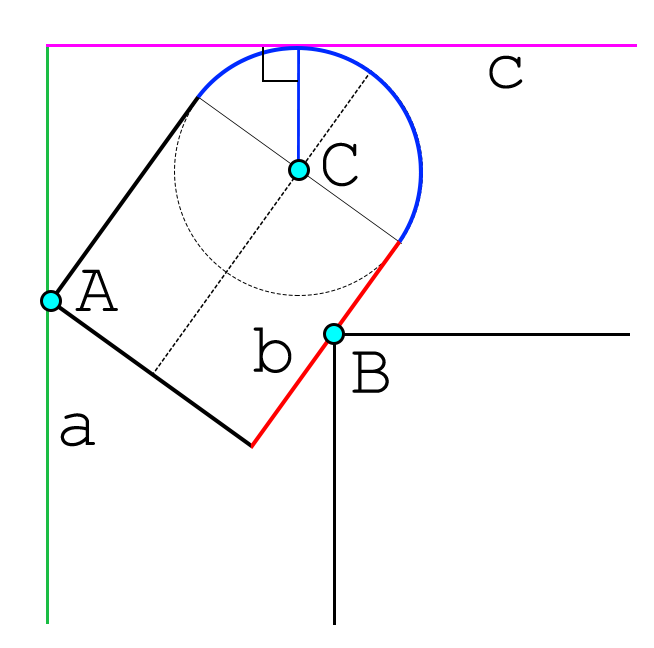
\includegraphics[width=6cm]{res/edges.png}
				\caption{Препятствия-ограничения}
			\end{figure}
			\begin{enumerate}
				\item Первой парой объектов, составляющих ограничение, являются точка-угол плота $A$ и прямая-стенка канала $a$ (выделена зеленым цветом).
				\item Следующая пара - точка-угол поворота $B$ и прямая-грань плота $b$ (выделена красным цветом).
				\item Последнее ограничение строится из соприкосновения носовой круглой части плота (выделена синим цветом) с центром в точке $C$ и прямой-стенки канала $c$ (выделена пурпурным цветом).
			\end{enumerate}
		
		\subsection{Построение модели}
			Проведя анализ в предыдущем пункте, можно свести модель перемещения двумерного плота в повороте к 3-ем тривиальным ограничениям расстояний между точками и прямыми:
			\begin{equation}\label{eq:limitations}
				\left\{
					\begin{array}{ll}
						\rho(A, a) >= 0,\\
						\rho(B, b) >= 0,\\
						\rho(C, c) >= a
					\end{array}
				\right.
			\end{equation}
			
			Объединяя все предыдущие рассуждения, начнем построение математической модели с установки системы координат. Для этого повернем нашу схему на 90 градусов против часовой стрелки и установим внешний угол канала в начало прямоугольной системы координат-точку $O(0,0)$.\\
			
			Также введем третью координату-угол $\varphi$, который отсчитывается, как это приведено на схеме ниже. Получаем тем самым левостороннюю СК:
			\begin{figure}[H]\label{fig:model}
				\centering
				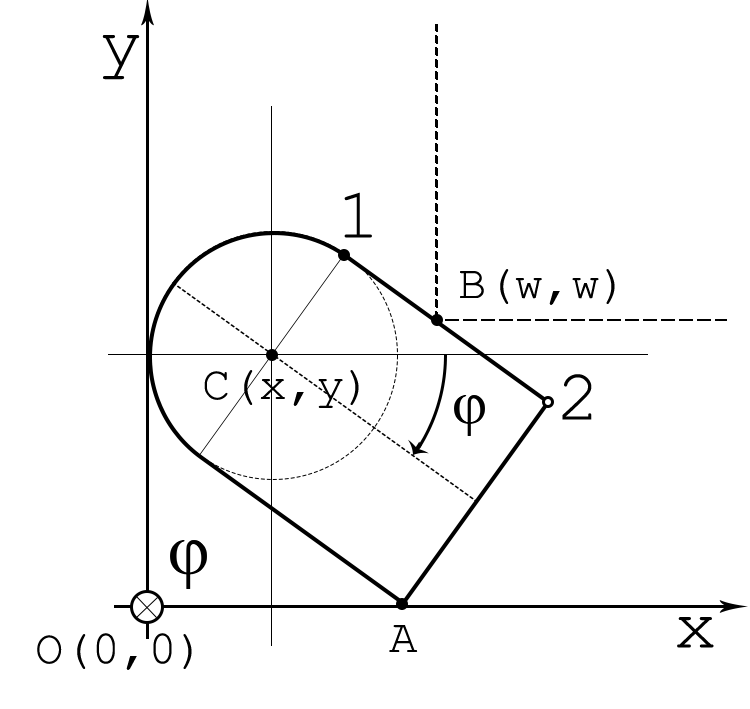
\includegraphics[width=10cm]{res/model.png}
				\caption{Математическая модель задачи}
			\end{figure}
			
			Приведем пояснения к построенной схеме:
			\begin{itemize}
				\item Сузим рассмотрение плоского твердого тела до размеров материальной точки $C$, являющейся центром полукруга плота. Можно считать, что данная точка имеет 3 координаты в нашей СК: $C(x, y, \varphi)$. Ясно, что такая точка с 3 заданными координатами взаимно однозначно соответствует положению плота в двумерном пространстве.
				\item Построенная СК позволяет свести систему 
				\eqref{eq:limitations} к более простому виду:
				\begin{equation}\label{eq:limitations_simplified}
					\left\{
						\begin{array}{ll}
							A_y >= 0,\\
							\rho(B, b) >= 0, \hskip 0.1 cm \mbox{где b - отрезок прямой с концами в точках 1 и 2}\\
							C_x >= a
						\end{array}
					\right.
				\end{equation}
				\item Из аналитической геометрии нам известно, что расстояние между точкой и прямой на плоскости вычисляется по формуле
				\begin{equation}
					d = \frac{|Mx_0 + Ny_0 + K|}{\sqrt{M^2 + N^2}},
				\end{equation}
				где\\
				$M, N, K$ - коэффициенты уравнения прямой в общем виде $Mx + Ny + K = 0$,\\
				$(x_0, y_0)$ - координаты точки.
				
				\newpage
				
				Мы также знаем, что величина $Mx_0 + Ny_0 + K$ принимает значения определенного знака в зависимости от взаимного расположения прямой и точки относительно начала координат. В нашем случае точка всегда находится за прямой относительно начала координат, поэтому это значение всегда должно быть $\geqslant 0$.
				\item Имея текущие значения $x, y, \varphi$, все необходимые в задаче координаты мы можем вычислить по следующим формулам:
				\begin{equation}\label{eq:formulas}
					\begin{array}{ll}
						A_x = x + a\sqrt{5}\cos(\varphi + \arctan{\frac{1}{2}})\\
						A_y = y - a\sqrt{5}\sin(\varphi + \arctan{\frac{1}{2}})\\
						1_x = x + a\sin\varphi\\
						1_y = y + a\cos\varphi\\
						2_x = x + a\sqrt{5}\cos(\varphi - \arctan{\frac{1}{2}})\\
						2_y = y - a\sqrt{5}\sin(\varphi - \arctan{\frac{1}{2}})
					\end{array}
				\end{equation}
				А также можем вычислить необходимые параметры прямой $|1, 2|$, если представить ее уравнение в общем виде $Mx + Ny + K = 0$:
				\begin{equation}
					\begin{array}{ll}
						M = 1_y - 2_y\\
						N = 2_x - 1_x\\
						K = 1_x 2_y - 2_x 1_y
					\end{array}
				\end{equation}
			\end{itemize}
		
	\section{Алгоритм и реализация решения}
		Предлагается решение данной задачи с помощью экспериментальных манипуляций построенной математической модели. Точнее - мы будем задавать начальное положение плота (зададим точку $C(x,y,\varphi)$) и с помощью решения вспомогательной задачи оптимизации попытаемся $"$прогнать$"$ его через поворот в канале.\\
		
		В качестве постановки вспомогательной задачи можно указать следующие данные:
		\begin{equation}\label{eq:aux}
			\begin{array}{ll}
				\mbox{Максимизировать функцию цели}\\
				-x + y + \varphi \longrightarrow \max\\
				\mbox{при следующих условиях:}
			\end{array}
			\\
			\left\{
				\begin{array}{ll}
					y - a\sqrt{5}\sin(\varphi + \arctan{\frac{1}{2}}) \geqslant \delta\\ \\ 
					\frac{Mw + Nw + K}{\sqrt{M^2 + N^2}} \geqslant \delta\\ \\
					x \geqslant a \\ \\
					x \in (a, w - a)\\ \\
					y \in (a, Y)\\ \\
					\varphi \in (0, \frac{\pi}{2})
				\end{array}
			\right.
		\end{equation}
		где\\
		первые 3 уравнения полностью соответствуют системе \eqref{eq:limitations_simplified} за исключением того, что во втором уравнении мы более не рассматриваем модуль расстояния,\\
		$a$-заданный параметр размеров плота,\\
		$w$-заданная ширина канала,\\
		$\delta$-некоторая малая величина,\\
		$Y$-некоторое наперед заданное значение координаты $y$, достижение которого точкой $C$ мы условно примем за успешное преодоление поворота.\\
		\textit{Замечание:} от третьего условия данной задачи можно избавиться, т.к. оно регулируется множеством допустимых значений координаты $x$.
		
		\newpage
		
		Понятно, что перед нами нелинейная задача условной оптимизации.\\
		Для ее решения был задействован алгоритм квадратичного программирования SLSQP из пакета scipy.optimize \hyperref[2]{[2]}, поставляемого для языка Python. Данный алгоритм как раз представляет из себя итерационный метод решения нелинейных задач условной оптимизации.\\
		
		Для данной работы, как уже было сказано выше, применялся экспериментальный подход, а именно задавалась некоторая последовательность значений параметра размеров плота $a$ в пределах $(\frac{w}{3}, \frac{w}{2})$ (см. \hyperref[subsec:limitations]{\textit{Ограничения}}) и устанавливалось приближенное граничное значение, при котором плот еще мог преодолеть поворот.\\
		
		Данный алгоритм поддерживает задание необходимой точности вычислений, а потому, вообще говоря, ничего не мешает реализовать алгоритм поиска приближенного решения относительно параметра $a\in(\frac{w}{3}, \frac{w}{2})$ с произвольной точностью.
	
	\section{Результаты}
		В качестве экспериментальной последовательности значений параметра размеров плота $a$ были выбраны следующие значения $\{0.333w, 0.400w, 0.437w, 0.438w, 0.460w, 0.499w\}$.\\
		
		Благодаря возможности вызова callback функции из метода SLSQP нам удается восстановить последовательность значений точки $(x,y,\varphi)$, построенной алгоритмом, и по данной последовательности восстановить графические интерпретации изменений математической модели. Приведем их для всей последовательности значений параметра:
		\begin{figure}[H]
			\centering
			\subfigure[$a=0.333w$]{
				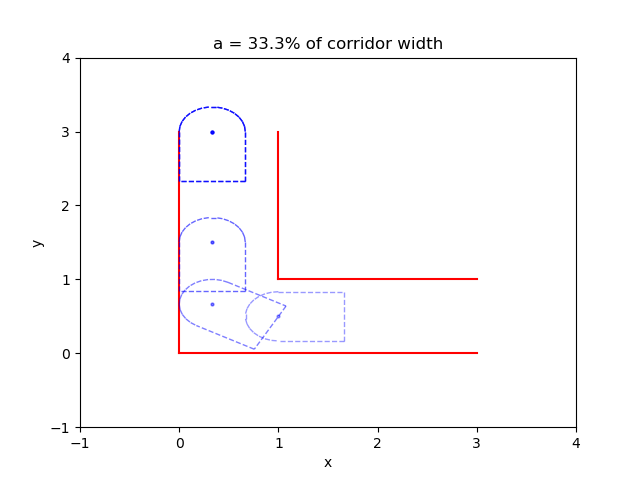
\includegraphics[width=0.48\linewidth]{res/out/0.333w.png}
			}
			\subfigure[$a=0.400w$]{
				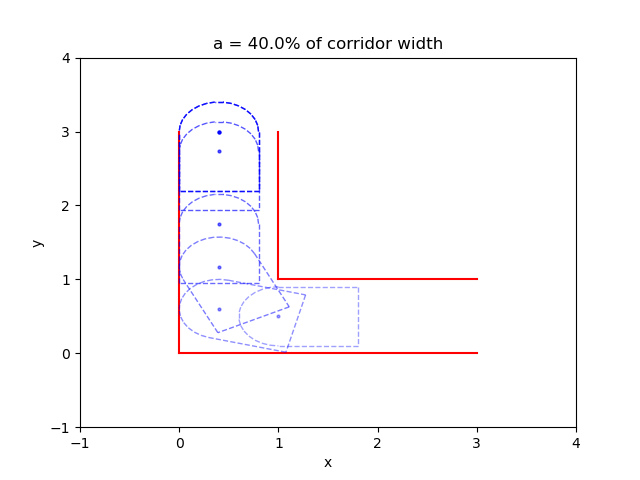
\includegraphics[width=0.48\linewidth]{res/out/0.400w.png}
			}
			\caption{Моделирование передвижения плота для $a = 0.333w$ и $a = 0.400$}
		\end{figure}
		\begin{figure}[H]
			\centering
			\subfigure[$a=0.437w$]{
				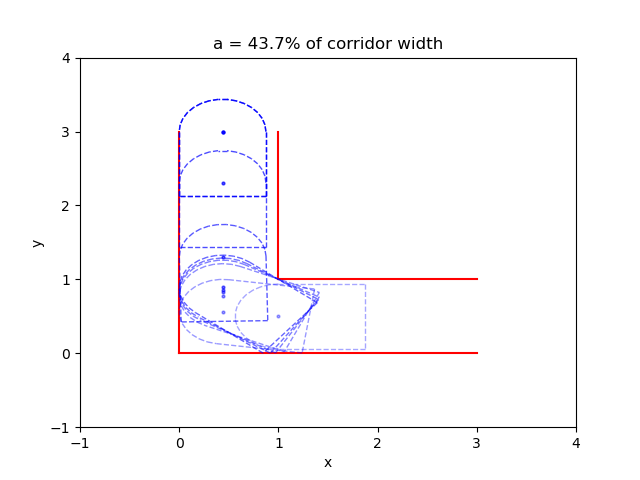
\includegraphics[width=0.48\linewidth]{res/out/0.437w.png}
			}
			\subfigure[$a=0.438w$]{
				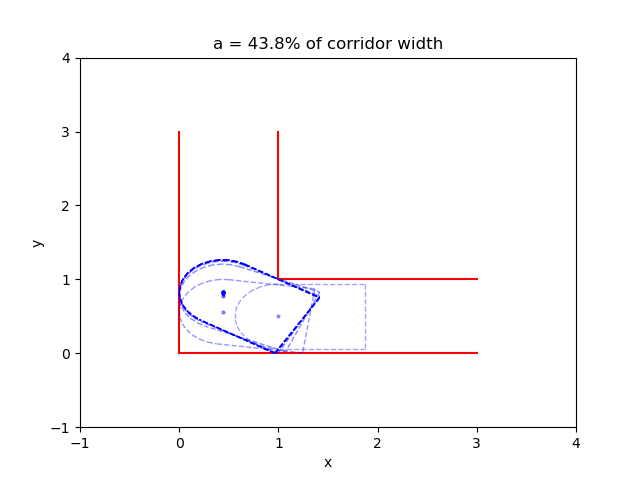
\includegraphics[width=0.48\linewidth]{res/out/0.438w.png}
			}
			\caption{Моделирование передвижения плота для $a = 0.437w$ и $a = 0.438$}
		\end{figure}
		\begin{figure}[H]
			\centering
			\subfigure[$a=0.460w$]{
				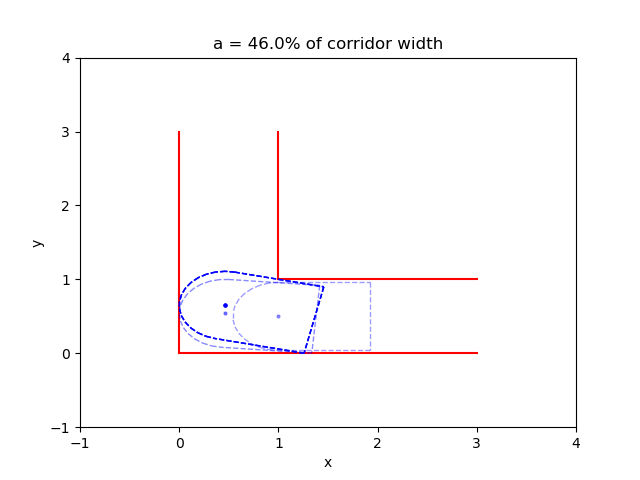
\includegraphics[width=0.48\linewidth]{res/out/0.460w.png}
			}
			\subfigure[$a=0.499w$]{
				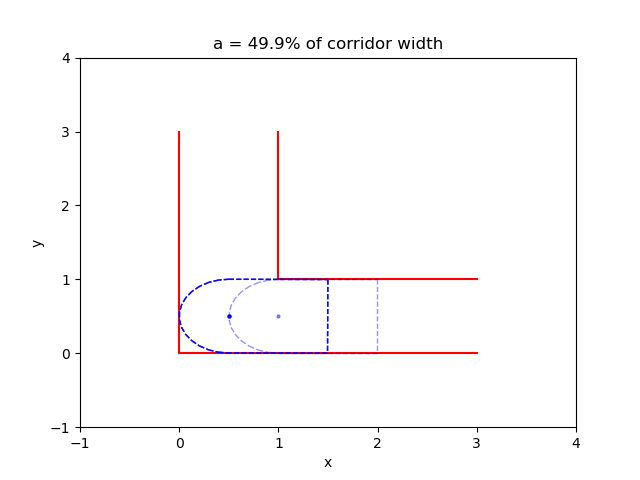
\includegraphics[width=0.48\linewidth]{res/out/0.499w.png}
			}
			\caption{Моделирование передвижения плота для $a = 0.460w$ и $a = 0.499$}
		\end{figure}
	
	Исходя из полученных результатов, можно сделать вывод, что с точностью $\sim1e-3$ значение параметра $a=0.437w$ является приближенным решением задачи.\\
	
	Таким образом максимальное значение площади фигуры данной конфигурации по формуле \eqref{eq:area} составляет: 
	\begin{equation}\label{eq:result}
		S = w^2 0.437^2 (4 + \frac{\pi}{2}) \approx 1.064w^2
	\end{equation}
	где $w$-заданная ширина канала\\
	
	\noindent Исходный код эксперимента приведен в \hyperref[sec:references]{\textit{ссылках}}.
	
	\newpage
	
	\section{Ссылки}\label{sec:references}
		\noindent [1]\label{1} Differential equations and exact solutions in the
		moving sofa problem, Dan Romik, 2016\\ {\url{https://www.math.ucdavis.edu/~romik/data/uploads/papers/sofa.pdf}}\\
		\vskip 0.1 cm
		\noindent [2]\label{2} Документация scipy.optimize для алгоритма SLSQP\\
		{\url{https://docs.scipy.org/doc/scipy/reference/optimize.minimize-slsqp.html}}\\
		\vskip 0.1 cm
		\noindent [3]\label{3} Репозиторий с исходным кодом эксперимента\\
		{\url{https://github.com/via8/MethOpt/tree/master/Course}}
\end{document}
